% Generated by pysimcount.figleader -- do not edit; regenerate instead.
% figure: main-total-all-formulas -- cost at n = 500, one row per formula
% seeds [1, 2, 3, 4, 5, 6, 7, 8, 9, 10]; metric=total kind=xyz merged (Clifford+Rz (cz), simcount template)
% shown: suzuki4, suzuki6, mo-q6, mo-q14, bm-q10, mo-o8-q21, morales-y8m10, morales-m8
% removed (see main-total-all-formulas-ranking.md): lie-trotter, suzuki2, suzuki8
% n = 500; x = the source record's plotted value; bars min..max over seeds
% cheapest on = seeds on which the formula is cheapest; rank range = min..max of its rank over seeds
% per-seed values: runs' totals if measured, else each seed's own fit c(n) ceil(a_s n^b_s)
% row order (plotted value) ['bm-q10', 'morales-m8', 'mo-q14', 'morales-y8m10', 'mo-q6', 'mo-o8-q21', 'suzuki6', 'suzuki4'] differs from mean-rank order ['morales-m8', 'bm-q10', 'mo-q14', 'morales-y8m10', 'mo-q6', 'mo-o8-q21', 'suzuki6', 'suzuki4']
% derived: main-total-all-formulas.json by pysimcount.figleader; source_sha256=30e50d3f6d86c0d6c6589486b4bbbbdd3558fc52ed6b877dec86feaaff7bef99
% figure made at git_commit=eed0c490bd2a7ed3c821acf76ae930c79d2195f6 git_dirty=False
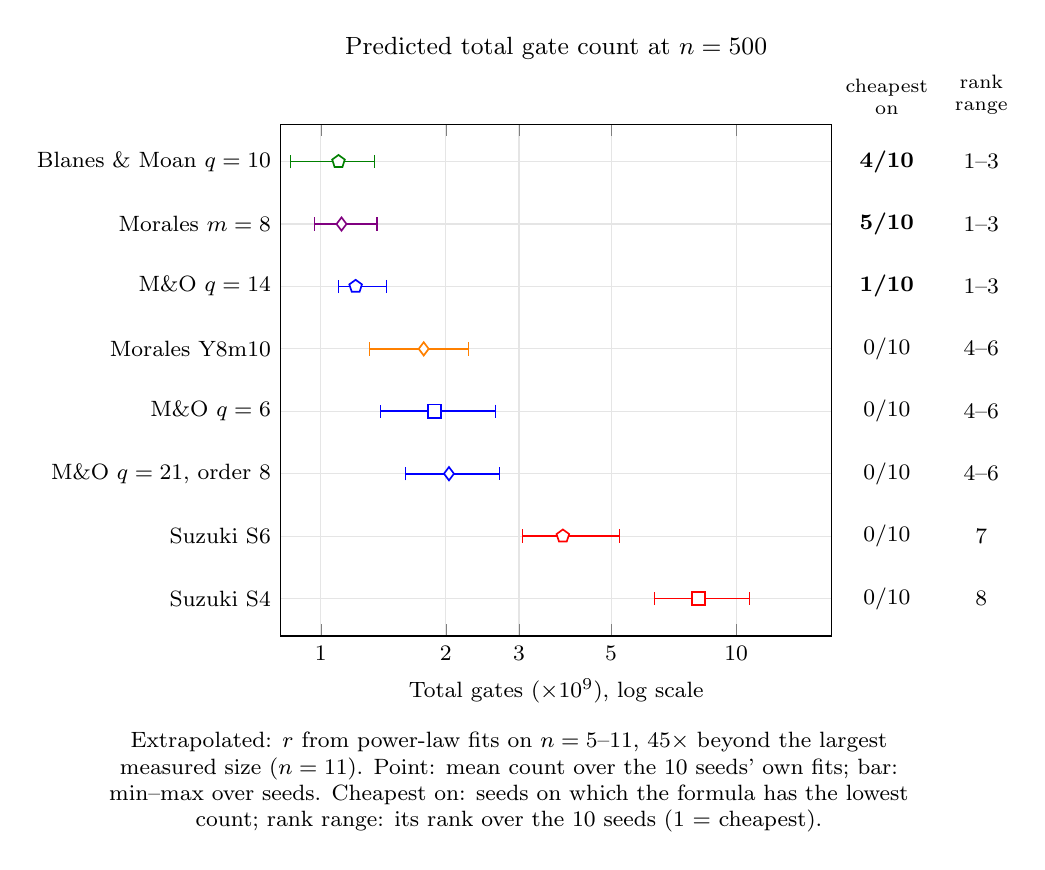
\begin{tikzpicture}
  \begin{semilogxaxis}[
    scale only axis, clip=false,
    at={(0cm,0cm)}, anchor=south west,
    width=7.0cm, height=6.5cm,
    title={Predicted total gate count at $n = 500$}, title style={font=\small, yshift=14pt},
    xlabel={Total gates ($\times 10^{9}$), log scale}, xlabel style={font=\footnotesize},
    xmin=8e+08, xmax=1.7e+10, xtick={1e+09,2e+09,3e+09,5e+09,1e+10}, xticklabels={1,2,3,5,10},
    xminorticks=false,
    y dir=reverse, ymin=0.4, ymax=8.6, ytick={1,2,3,4,5,6,7,8},
    yticklabels={{Blanes \& Moan $q=10$},{Morales $m=8$},{M\&O $q=14$},{Morales Y8m10},{M\&O $q=6$},{M\&O $q=21$, order 8},{Suzuki S6},{Suzuki S4}},
    tick label style={font=\footnotesize}, ytick style={draw=none},
    xmajorgrids=true, ymajorgrids=true, grid style={black!10},
  ]
    % bm-q10: plotted 1.10288e+09, seeds 8.43591e+08..1.34816e+09, cheapest on 4/10, rank 1..3
    \addplot[green!50!black, only marks, mark=pentagon*, mark size=2.4pt, mark options={solid, fill=white, line width=0.6pt}, error bars/.cd, x dir=both, x explicit, error bar style={solid, line width=0.6pt}] coordinates {
      (1.10288e+09,1) += (2.45279e+08,0) -= (2.59291e+08,0)
    };
    % morales-m8: plotted 1.12147e+09, seeds 9.65888e+08..1.36541e+09, cheapest on 5/10, rank 1..3
    \addplot[violet, only marks, mark=diamond*, mark size=2.4pt, mark options={solid, fill=white, line width=0.6pt}, error bars/.cd, x dir=both, x explicit, error bar style={solid, line width=0.6pt}] coordinates {
      (1.12147e+09,2) += (2.43936e+08,0) -= (1.55584e+08,0)
    };
    % mo-q14: plotted 1.21287e+09, seeds 1.10187e+09..1.43739e+09, cheapest on 1/10, rank 1..3
    \addplot[blue, only marks, mark=pentagon*, mark size=2.4pt, mark options={solid, fill=white, line width=0.6pt}, error bars/.cd, x dir=both, x explicit, error bar style={solid, line width=0.6pt}] coordinates {
      (1.21287e+09,3) += (2.24527e+08,0) -= (1.11e+08,0)
    };
    % morales-y8m10: plotted 1.76907e+09, seeds 1.31025e+09..2.27156e+09, cheapest on 0/10, rank 4..6
    \addplot[orange, only marks, mark=diamond*, mark size=2.4pt, mark options={solid, fill=white, line width=0.6pt}, error bars/.cd, x dir=both, x explicit, error bar style={solid, line width=0.6pt}] coordinates {
      (1.76907e+09,4) += (5.02485e+08,0) -= (4.58825e+08,0)
    };
    % mo-q6: plotted 1.87899e+09, seeds 1.39555e+09..2.63917e+09, cheapest on 0/10, rank 4..6
    \addplot[blue, only marks, mark=square*, mark size=2.4pt, mark options={solid, fill=white, line width=0.6pt}, error bars/.cd, x dir=both, x explicit, error bar style={solid, line width=0.6pt}] coordinates {
      (1.87899e+09,5) += (7.60176e+08,0) -= (4.83445e+08,0)
    };
    % mo-o8-q21: plotted 2.03494e+09, seeds 1.59669e+09..2.69123e+09, cheapest on 0/10, rank 4..6
    \addplot[blue, only marks, mark=diamond*, mark size=2.4pt, mark options={solid, fill=white, line width=0.6pt}, error bars/.cd, x dir=both, x explicit, error bar style={solid, line width=0.6pt}] coordinates {
      (2.03494e+09,6) += (6.56295e+08,0) -= (4.38253e+08,0)
    };
    % suzuki6: plotted 3.82702e+09, seeds 3.05936e+09..5.23534e+09, cheapest on 0/10, rank 7..7
    \addplot[red, only marks, mark=pentagon*, mark size=2.4pt, mark options={solid, fill=white, line width=0.6pt}, error bars/.cd, x dir=both, x explicit, error bar style={solid, line width=0.6pt}] coordinates {
      (3.82702e+09,7) += (1.40832e+09,0) -= (7.67653e+08,0)
    };
    % suzuki4: plotted 8.12156e+09, seeds 6.37431e+09..1.07703e+10, cheapest on 0/10, rank 8..8
    \addplot[red, only marks, mark=square*, mark size=2.4pt, mark options={solid, fill=white, line width=0.6pt}, error bars/.cd, x dir=both, x explicit, error bar style={solid, line width=0.6pt}] coordinates {
      (8.12156e+09,8) += (2.64878e+09,0) -= (1.74725e+09,0)
    };
    \node[anchor=south, font=\scriptsize, align=center] at ([xshift=0.7cm]axis cs:1.7e+10,0.4) {cheapest\\on};
    \node[anchor=south, font=\scriptsize, align=center] at ([xshift=1.9cm]axis cs:1.7e+10,0.4) {rank\\range};
    \node[font=\footnotesize\bfseries] at ([xshift=0.7cm]axis cs:1.7e+10,1) {4/10};
    \node[font=\footnotesize] at ([xshift=1.9cm]axis cs:1.7e+10,1) {1--3};
    \node[font=\footnotesize\bfseries] at ([xshift=0.7cm]axis cs:1.7e+10,2) {5/10};
    \node[font=\footnotesize] at ([xshift=1.9cm]axis cs:1.7e+10,2) {1--3};
    \node[font=\footnotesize\bfseries] at ([xshift=0.7cm]axis cs:1.7e+10,3) {1/10};
    \node[font=\footnotesize] at ([xshift=1.9cm]axis cs:1.7e+10,3) {1--3};
    \node[font=\footnotesize] at ([xshift=0.7cm]axis cs:1.7e+10,4) {0/10};
    \node[font=\footnotesize] at ([xshift=1.9cm]axis cs:1.7e+10,4) {4--6};
    \node[font=\footnotesize] at ([xshift=0.7cm]axis cs:1.7e+10,5) {0/10};
    \node[font=\footnotesize] at ([xshift=1.9cm]axis cs:1.7e+10,5) {4--6};
    \node[font=\footnotesize] at ([xshift=0.7cm]axis cs:1.7e+10,6) {0/10};
    \node[font=\footnotesize] at ([xshift=1.9cm]axis cs:1.7e+10,6) {4--6};
    \node[font=\footnotesize] at ([xshift=0.7cm]axis cs:1.7e+10,7) {0/10};
    \node[font=\footnotesize] at ([xshift=1.9cm]axis cs:1.7e+10,7) {7};
    \node[font=\footnotesize] at ([xshift=0.7cm]axis cs:1.7e+10,8) {0/10};
    \node[font=\footnotesize] at ([xshift=1.9cm]axis cs:1.7e+10,8) {8};
  \end{semilogxaxis}
  \node[anchor=north, text width=10.5cm, align=flush center, font=\footnotesize] at (2.9cm,-1.1cm) {Extrapolated: $r$ from power-law fits on $n = 5$--$11$, 45$\times$ beyond the largest measured size ($n = 11$). Point: mean count over the 10 seeds' own fits; bar: min--max over seeds. Cheapest on: seeds on which the formula has the lowest count; rank range: its rank over the 10 seeds (1 = cheapest).};
\end{tikzpicture}
